\chapter{Aplicații WebRTC}
\label{chap:ch4}

\section{Microsoft Teams}
\label{chap:ch4sec1}
\begin{figure}[!htbp]
    \centering
    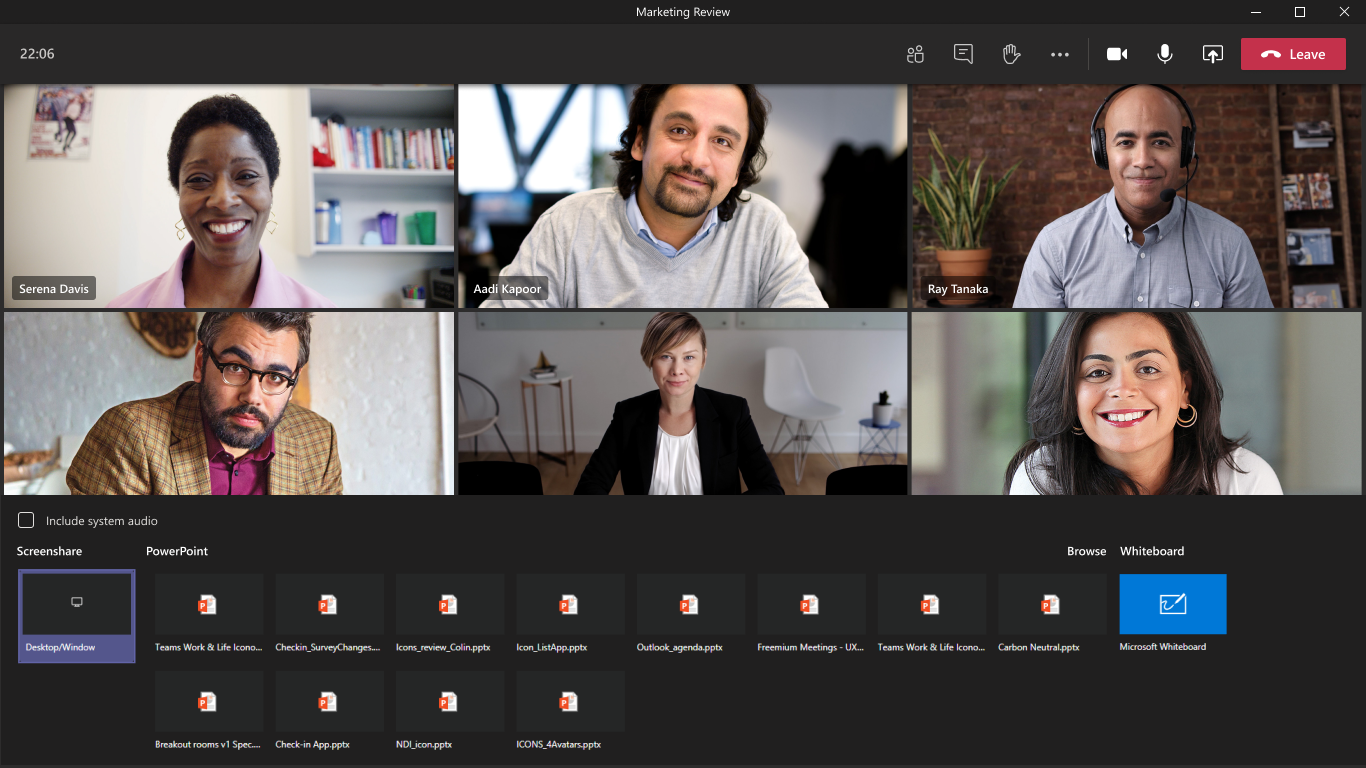
\includegraphics[width=12cm]{figures/ms_teams_call.png}
    \caption{Conversație pe Teams}
\end{figure}

\indent \par Aplicația propriu-zisă a fost implementată inițial folosind framework-ul Angular. În 2018, Abhik Mitra a propus migrarea treptată către React \cite{TeamsReact2018}, astfel că dezvoltatorii pot crea în zilele noastre aplicații pentru Teams folosind componente React puse la dispoziție de Microsoft.
\indent \par Teams este conceput pentru a fi folosit în mediul profesional, în care există posibilitatea ca angajații să folosească VPN-uri, ca unii clienți să folosească Skype for Business și/sau să participe dintr-o rețea externă companiei sau chiar de pe o linie telefonică obișnuită, prin rețeaua PSTN. Pentru a putea face conversația în aceste cazuri posibilă, Microsoft a implementat o serie de mecanisme de redistribuire a streamurilor media. Transport relay-ul este un server STUN, folosit pentru a obține candidații ICE, și este parte a suitei Microsoft 365. Va funcționa ca releu media, asemenea serverului TURN, în cazul în care un participant nu se află în aceeași rețea. Protocolul de signaling folosit este preponderent HTTPS, prin servicii REST \cite{TeamsFlows2018}, însă va folosi și SIP pentru a interacționa cu SBC-uri (session border controller).
\begin{figure}[!htbp]
    \centering
    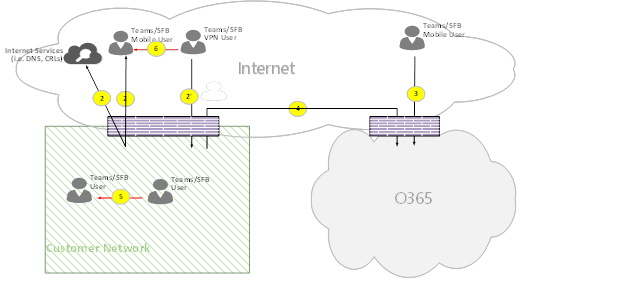
\includegraphics[width=11cm]{figures/ms_teams_topology.png}
    \caption{Topologia de rețea folosită în apelurile Microsoft Teams în care toți participanții folosesc Teams}
\end{figure}
\indent \par Pentru a face posibile conversațiile pe Teams prin linia telefonică, Microsoft pune la dispoziție așa numitul Phone System prin abonamentul Microsoft 365, care este un private branch exchange (PBX), o centrală telefonică.
\begin{figure}[!htbp]
    \centering
    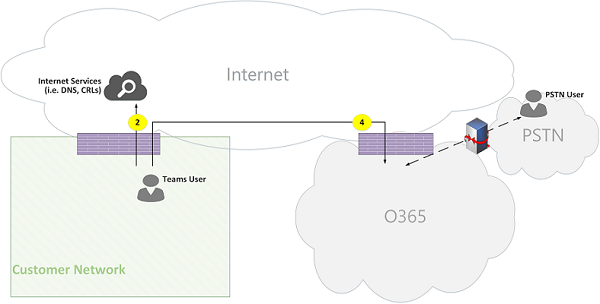
\includegraphics[width=11cm]{figures/ms_teams_to_pstn.png}
    \caption{Topologia unei conversații între un utilizator Teams și un utilizator al liniei telefonice obișnuite}
\end{figure}

\section{Jitsi Meet}
\label{chap:ch4sec2}
\begin{figure}[!htbp]
    \centering
    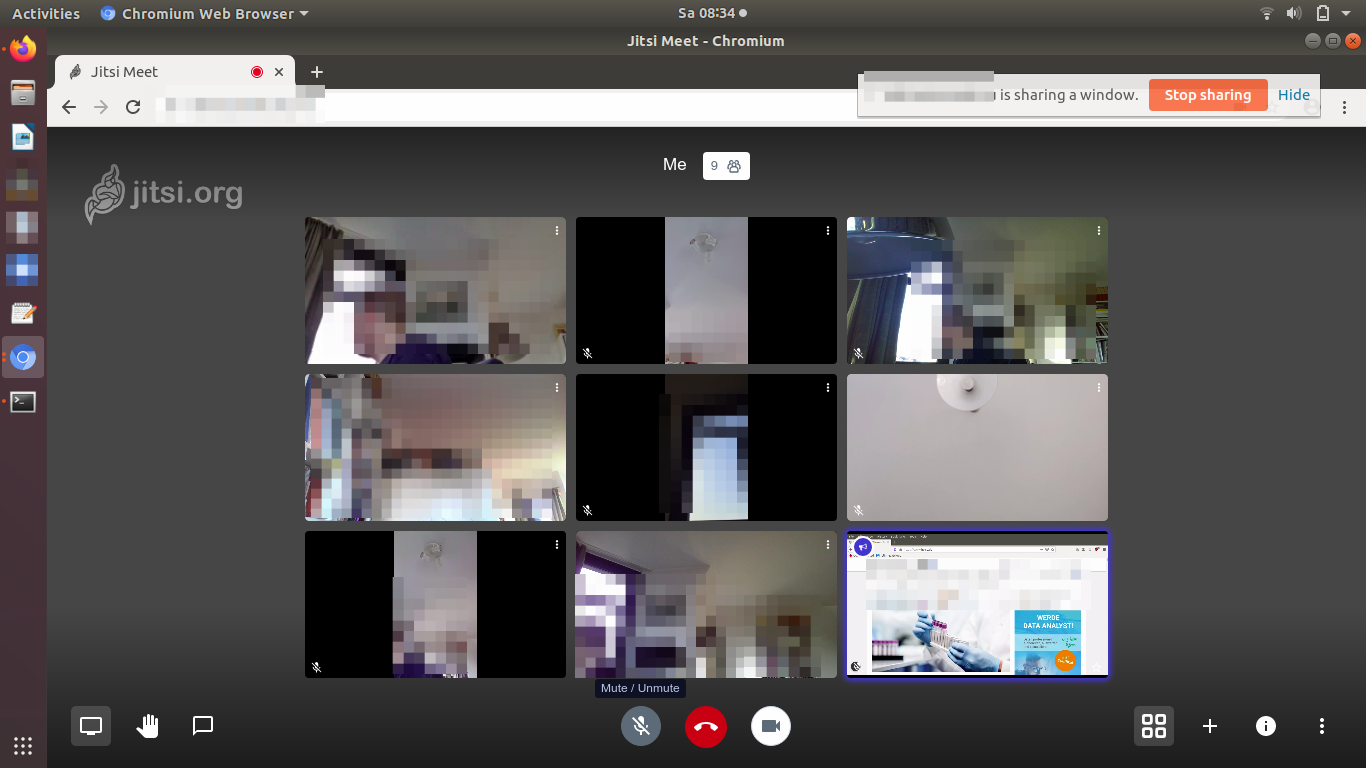
\includegraphics[width=11cm]{figures/jitsi_meet_call.png}
    \caption{Conversație pe Jitsi}
\end{figure}
\indent \par Jitsi Meet este o aplicație open-source implementată, de asemenea, cu WebRTC. Asociat acestei aplicații este Jitsi Videobridge, un server SFU ce suportă simulcast și care este considerat mai eficient decât un MCU. Oricine poate să îl instaleze local. Signaling-ul va fi realizat folosind un server Prosody prin protocolul XMPP \cite{JitsiArchitecture}.
\indent \par Teste de performanță au fost făcute pe o configurație cu un procesor quad-core Intel Xeon E5-1620 v2 la 3,7 GHz. S-a observat că o dată cu creșterea lățimii de bandă folosite, consumul de resurse a crescut liniar \ref{JitsiVideobridgeCPU}.  Folosind 33 de clienți (load generators), serverul a distribuit 1056 de streamuri, iar lățimea de bandă folosită a ajuns la 550 Mbps \ref{JitsiVideobridgeBandwidth} \cite{JitsiVideobridge}. 20\% din capacitatea procesorului a fost folosită, conform datelor furnizate de procesul \textit{top} \cite{JitsiVideobridge}.
\begin{figure}[H]
    \centering
    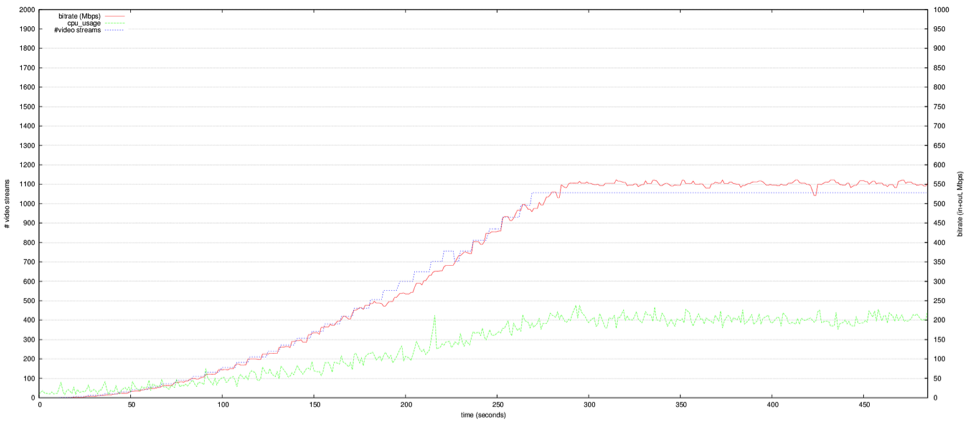
\includegraphics[width=15cm]{figures/jitsi_videobridge_bandwidth.png}
    \caption{Grafic pentru lățimea de bandă folosită direct proporțională cu numărul de streamuri}
    \label{JitsiVideobridgeBandwidth}
\end{figure}
\begin{figure}[H]
    \centering
    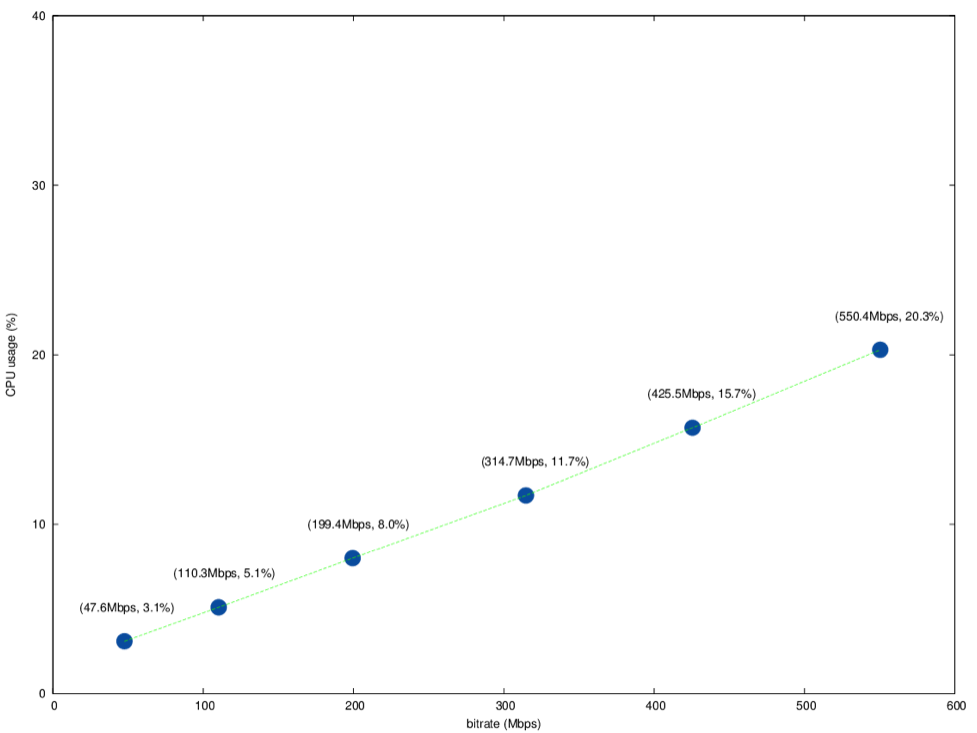
\includegraphics[width=11cm,trim={0 0 0 3cm}, clip]{figures/jitsi_videobridge_cpu.png}
    \caption{Grafic al capacității procesorului folosite în funcție de lățimea de bandă}
    \label{JitsiVideobridgeCPU}
\end{figure}
\indent \par Deoarece pot fi mulți participanți într-o conferință, s-a creat Jicofo (Jitsi Conference Focus), care are rolul de load balancing între fiecare participant și Videobridge \cite{JitsiArchitecture}.
\indent \par În cazul participanților din diferite zone geografice, aceștia se vor conecta la cel mai apropiat SFU (bridge), urmând ca serverele la care s-au conectat clienții să își transmită reciproc stream-urile \cite{JitsiBridgeCascading}. Această tehnică se numește bridge cascading \cite{JitsiBridgeCascading}.

\section{Zoom}
\label{chap:ch4sec3}

\begin{figure}[!htbp]
    \centering
    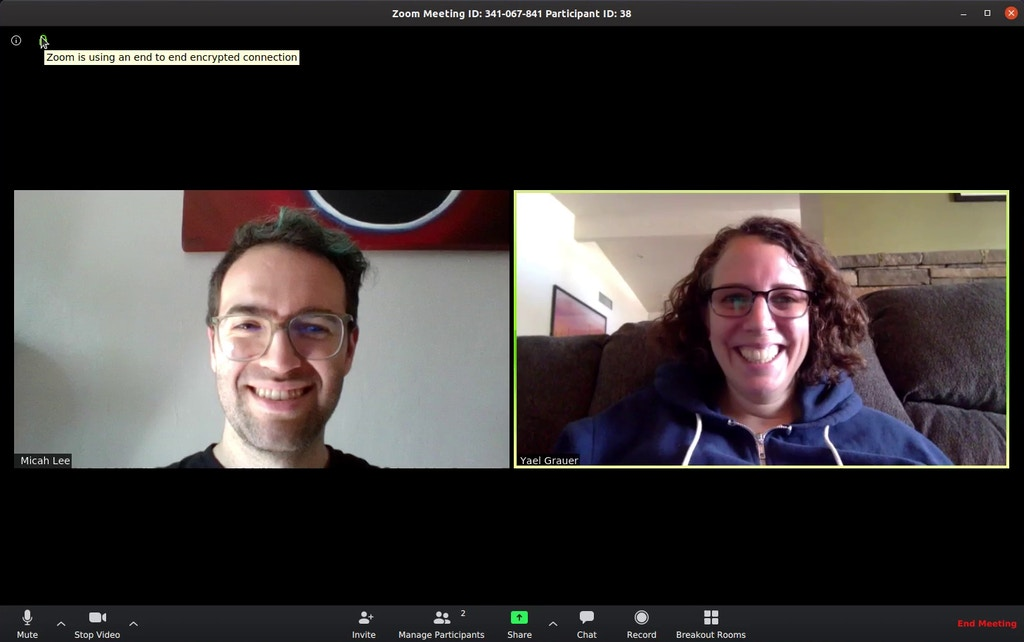
\includegraphics[width=13cm]{figures/zoom_call.jpg}
    \caption{Conversație pe Zoom}
\end{figure}
\indent \par Spre deosebire de alte platforme de videoconferințe, Zoom folosește o implementare care se bazează pe RTCDataChannel și nu pe protocolul RTP \cite{ZoomWebRTC}. Conținutul video folosește codecul H.264 Annex G, care permite o scalabilitate mai bună datorită codării stratificate și pe care browserul Chrome nu îl suportă nativ \cite{ZoomScalability, ZoomWebRTC}. așadar, include furnizează un codec special compilat în WebAssembly \cite{ZoomWebRTC}.
\indent \par Zoom folosește un router multimedia care separă conținutul ce trebuie transcodat și procesat de cel care trebuie pur și simplu redistribuit, ceea ce îi oferă un avantaj real în privința scalabilității și a consumului de resurse \cite{ZoomScalability}.
\indent \par Nu folosește server STUN sau TURN, dovada fiind lista \textit{iceServers} goală din configurația obiectului RTCPeerConnection \cite{ZoomWebRTC}. În cazul în care nu se poate folosi UDP (ex.: este blocat pe firewall), va folosi implementarea veche pe bază de WebSocket, încercând să instanțieze un nou obiect RTCPeerConnection la fiecare 10 secunde \cite{ZoomWebRTC}.
\begin{figure}[!htbp]
    \centering
    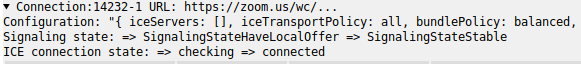
\includegraphics[width=14cm]{figures/zoom_no_ice_servers.png}
    \caption{Configurația folosită de clientul web Zoom}
\end{figure}
\indent \par Zoom, de asemenea, manipulează descriptorul creat folosind funcția \textit{createOffer} înainte să îl seteze ca fiind cel local. Va schimba username fragment-ul candidaților (prezent în SDP ca \texttt{a=ice-ufrag}) dintr-unul scurt, generat de Chrome, cu un UUID lung \cite{ZoomWebRTC}. Folosește specificația \textit{ice-lite}, o versiune minimală a protocolului ICE, marcată în SDP ca \texttt{a=ice-lite}.